\documentclass[tikz]{standalone}
\usepackage{pgfplots}
\pgfplotsset{compat=1.18}
\begin{document}
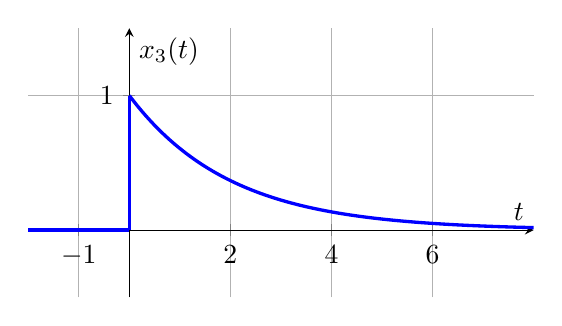
\begin{tikzpicture}
	\begin{axis}[
		width=8cm, height=5cm,
		axis lines=middle,
		xmin=-2, xmax=8, ymin=-0.5, ymax=1.5,
		xlabel={$t$}, ylabel={$x_3(t)$},
		grid=both,
		grid style={line width=.1pt, draw=gray!40},
		major grid style={line width=.2pt,draw=gray!60},
		xtick={-1,0,2,4,6}, ytick={0,1},
		samples=100
	]
	\addplot[line width=1.2pt, blue] coordinates {(-2,0) (0,0)};
	\addplot[line width=1.2pt, blue] coordinates {(0,0) (0,1)};
	\addplot[line width=1.2pt, blue, domain=0:8, samples=100] {exp(-x/2)};
	\end{axis}
\end{tikzpicture}
\end{document}
